\setchapterimage[6cm]{seaside}
\setchapterpreamble[u]{\margintoc}
\chapter{Introduction}
\labch{intro_observational}

\section{Equality in Intensional Type Theory}

If you have ever used a proof assistant based on intensional type theory such as
\Coq, \Agda or {\Lean} -- and there is a good chance that you have if you are 
reading this thesis -- then you probably know that equality can be a real headache.

On the one hand we have the \emph{definitional} equality (also called conversion), which records the 
equations that the proof assistant handles silently for us.
% 
\sideremark{In proof assistants based on ZF set theory such as Metamath,
  the theorem \( 2+2=4 \) does requires a proof. Although it is elementary,
  this proof involves hundreds of auxiliary lemmas!}
% 
For instance, the terms \( 2+2 \) and \( 4 \) are definitionally equal, meaning that we 
can use them interchangeably in our proofs without having to worry about 
proving their equality by hand.
% 
In a dependently typed setting, this minimal amount of automation is absolutely vital; 
lest we have to insert explicit coercions every time we want to say, use a term 
of type \( \mathsf{Vector}\ (2+2) \) as a term of type \( \mathsf{Vector}\ 4 \).

But unfortunately not everything is a natural 
number\sidenote{[citation needed]}, and mathematical proofs
frequently deal with equalities between infinitary objects such as functions and 
sets.
% 
And of course there is no algorithm that can decide whether
two functions of type \( \Nat \to \Nat \) are pointwise equal.
% 
Thus in practice, the definitional equality is limited to 
\( \beta / \eta / \iota \) equalities, with perhaps some extensions
such as \Agda's rewrite rules~\sidecite{taming_of_the_rew}.

Since the system will not be able to fully automate all equalities away, 
we need facilities to reason about them.
% 
This is why intensional type theories provide a second notion of equality, 
called the \emph{propositional} equality. 
% 
Contrary to the definitional equality, this one is available internally in
the language of type theory, so that we may use it to state and prove theorems.
% 
In all three major proof assistants based on type theory, the propositional 
equality is implemented as an inductive type, after the pioneer work of Martin-Löf~\sidecite{MartinLoef75}.
% 
\sideremark{The propositional equality \( \Indeq{A}{t}{u} \) is a type, while the
  definitional equality \( \eqtm{\Gamma}{t}{u}{A} \) is a typing judgment.}
\begin{mathpar}
  \inferrule{\tyty{\Gamma}{A}
			\\ \tytm{\Gamma}{t}{A}
			\\ \tytm{\Gamma}{u}{A}}
			{\tyty{\Gamma}{\Indeq{A}{t}{u}}}
  \and
  \inferrule{\tyty{\Gamma}{A}
			\\ \tytm{\Gamma}{t}{A}}
			{\tytm{\Gamma}{\indrefl{t}}{\Indeq{A}{t}{t}}}
\end{mathpar}
\begin{mathpar}
  \inferrule{\tyty{\Gamma}{A}
			\\ \tytm{\Gamma}{t}{A}
			\\ \tytm{\Gamma}{B}{\Depfun{A}{\Fun{t =_A x}{\Univ}}}
			\\ \tytm{\Gamma}{u}{B\ t\ \mathsf{refl}_t}
			\\ \tytm{\Gamma}{t'}{A}
			\\ \tytm{\Gamma}{e}{t =_A t'}}
			{\tytm{\Gamma}{\mathsf{J}(A,t,B,u,t',e)}{B\ t'\ e}}
\end{mathpar}
\begin{mathpar}
  \inferrule{[...]}
			{\red{\Gamma}{\mathsf{J}(A,t,B,u,t,\mathsf{refl}_t)}{u}{B\ t\ \mathsf{refl}_t}}
\end{mathpar}

These few rules are enough to define an equivalence relation that contains
the definitional equality, can be used to rewrite terms and can be used to coerce
between equal types.
%  (using the \( \mathsf{J} \) operator).

An important difference with the common practice of mathematics is the 
attachment to the Curry-Howard correspondence between proofs and programs:
equality is a \emph{type}, and equality proofs are \emph{programs}\sidenote{amen.}.
% 
As such, equality proofs are first class values like the natural numbers
or the functions, and we can reason about them or evaluate them just as well.

\subsection{Types and Propositions}

While the possibility to evaluate proofs is a core tenet of the Curry-Howard
doctrine, the typical equality proof does not exhibit a very interesting 
computational behavior. 
% 
The term \( \indJ{A}{t}{P}{u}{t'}{e} \) just waits for \( e \) to reduce to
a proof by reflexivity, in which case \( t \) and \( t' \) are convertible and
the whole term can simply evaluate to \( u \). 

As a consequence, the programs 
\defnote{extracted}{Extraction produces a program in an external programming 
  language by erasing type information.} 
from proofs that use equational reasoning  tend to spend a lot of time passing 
around equality proofs just to end up discarding them.
% 
This less-than-ideal state of affairs led the \Coq proof assistant to introduce
a special sort \( \varProp \) for types whose proofs are to be erased during 
program extraction~\sidecite{letouzey04}.
% 
By putting the propositional equality in \( \varProp \) along with the other logical 
constraints that do not play any role in computation, \Coq recovers reasonably good 
performances for extracted programs. 

Technically this is a bit of an infrigement of the Curry-Howard discipline, as \( \varProp \) 
effectively re-introduces a separation between propositions and data.
% 
But do not be mistaken: proofs of propositions still play their normal role in computations, and in 
particular they may block the evaluation of open terms. 
% 
It is only when we extract an \emph{external} program that propositions become irrelevant.

The \Lean proof assistant goes a step further and introduces the sort 
% 
\sideremark{The \Lean community uses the name \( \varProp \) for the sort of
  strict propositions, but we will use \( \varsProp \) to avoid confusion with
  non-strict propositions.}
% 
\( \varsProp \) for \emph{strict propositions}~\sidecite{lean}.
% 
% \sideremark{Nowadays strict propositions are also available in \Coq and
%   \Agda, although they do not use them for the propositional equality.}
% 
Contrary to \Coq's propositions, the strict propositions are proof-irrelevant, 
meaning that any two inhabitants of a strict proposition \( A \) are 
definitionally equal simply by virtue of having type \( A \).
% 
\[
\inferrule{\tytm{\Gamma}{A}{\varsProp} \\ \tytm{\Gamma}{t, u}{A}}{\eqtm{\Gamma}{t}{u}{A}}
\]

Putting the propositional equality in \( \varsProp \) is not exactly innocuous.
% 
It means that any proof of propositional equality between two convertible 
terms is now undistinguishable from a proof by reflexivity since they have the 
same type.
% 
In other words \Lean satisfies a strict version of the principle of \emph{uniqueness 
of identity proofs} (UIP).

Now non-reflexive equality proofs can't block computation anymore: the term
\( \indJ{A}{t}{P}{u}{t}{e} \) is convertible to 
\( \indJ{A}{t}{P}{u}{t}{\indrefl{t}} \), which should reduce!
% 
As a consequence, the \( J \) eliminator of \Lean reduces whenever it is applied to 
definitionally equal terms.
\begin{mathpar}
  \inferrule[J-conv]{[...] \\ \eqtm{\Gamma}{t}{t'}{A}}
			{\red{\Gamma}{\mathsf{J}(A,t,B,u,t',e)}{u}{B\ t'\ e}}
      \ilabel{infrule:J-conv}
\end{mathpar}

But while this rule is logically sound, Abel and Coquand showed that it leads to a 
failure of normalization for open terms~\cite{lmcs:6606}.
% 
\sideremark{It is known that \Lean's definitional equality is undecidable for
  other, independent reasons~\cite{gilbert:hal-01859964}. But this certainly
  did not prevent the \Lean community from developing a large amount of 
  mathematics.}
% 
Since the algorithms we use to check for convertibility rely on normalization, it 
follows that adding rule~\nameref{infrule:J-conv} breaks our decision procedures
for the definitional equality.
% 
As noted by Abel and Coquand, it is not clear whether this stems from a 
fundamental incompatibility between impredicative strict propositions and the 
propositional equality, or if a more clever strategy could solve this problem.

\subsection{Impredicativity}

In dependent type theory, a sort is said to be \emph{impredicative} if it is 
closed under dependent products over any index type. 
% 
For instance the sort of \Coq propositions is impredicative, because for all 
types \( A \) and functions \( \tm{B}{A \to \varProp} \) the dependent product 
\( \Depfun{A}{B\ x} \) is in \( \varProp \).
% The same goes for \Lean's strict propositions.

Impredicativity allows some amount of self-reference into the type system: 
we can use it to form a proposition \( P \) which quantifies over the type 
\( \varProp \) of all propositions, a type that contains \( P \).
% 
A classic example is the impredicative encoding of the false proposition.
\[
\Depfun[X]{\varProp}{X} \quad : \quad \varProp
\]

Compare this situation with the \emph{predicative} hierarchy 
$(\varType_i)_{i \in \Nat}$ 
% 
\sideremark{In the case of \Coq the predicative universes are technically not
  indexed by integers, but the system maintains a graph of level constraints that
  effectively does the same job.}
% 
of non propositional types.
In the non-propositional world, dependent products are forced to inhabit a 
universe level that is higher than both the level of their domain and the level
of their codomain:
% 
given a type \( A : \varType_i \) and a function \( {\tm{B}{A \to \varType_j}} \), 
their dependent product \( \Depfun{A}{B\ x} \) is in 
\( \varType_{\mathsf{max}(i,j)} \).
 
Predicativity removes the possibility for self-reference: if we try to 
replicate the encoding of the false proposition in \( \varType_0 \), the
resulting type lands in the next universe.
\[
\Depfun[X]{\varType_0}{X} \quad : \quad \varType_1
\]

Playing with self-reference is always a dangerous game: 
logical antinomies born of Russell's paradox are lurking in the shadows, and 
might catch us if we get a bit too greedy with our logical principles. 
% 
For instance, Berardi's paradox shows that having excluded middle and booleans
with large elimination in \( \varProp \) is inconsistent.
% 
Impredicativity also plays a central role in the non-normalizing term
that Abel and Coquand derived from rule~\nameref{infrule:J-conv}~\sidecite{lmcs:6606}.

In counterpart to this fragility, impredicativity greatly increases the
expressive power of our logical system, and allows us to formulate important 
mathematical constructions such as Tarski's fixed point theorem or nontrivial 
complete lattices~\sidecite{paco}.
% 
Plus some theorems such as the normalization of System F outright cannot be 
proved in a predicative theory.

Different proof assistants have adopted different attitudes toward 
impredicativity.
% 
On the one hand,
% 
\sideremark{Back in the day the \Coq proof assistant used impredicative sorts
  for both computational data and proofs, but the development team switched to a 
  theory that is more compatible with classical mathematics.}
% 
\Coq and \Lean both have an impredicative sort for propositions, in 
parallel to the predicative universe hierarchy for the computationally 
relevant types~\sidecite{Coq:manual,lean}.
%
On the other hand, the \Agda proof assistant does not support impredicativity
and uses two predicative hierarchies instead, one for strict propositions and 
one for types~\sidecite{agda261}.

\section{Recovering Extensionality in Intensional Type Theory}

The basic propositional equality that we defined as an inductive type does 
not quite meet the standards of mathematical reasoning.
% 
In mathematics, two functions are considered equal when they agree on all 
inputs -- this is the principle of \emph{function extensionality} --
% 
\sideremark{In particular, it is not possible to prove that the functions
\( {\lambda\ n\ .\ n+1} \) and \( {\lambda\ n\ .\ 1+n} \) are equal.}
% 
but this principle is not derivable for the propositional equality in 
intensional type theory.
\[
  \Indeq{A \to B}{f}{g} \quad \xcancel{\longleftrightarrow} \quad \Depfun{A}{\Indeq{B}{f\ x}{g\ x}}
\]

In fact, we can show that all proofs of propositional equality in an empty 
context reduce to the definitional equality.
% 
This is a straightforward consequence of the normalization of well-typed terms:
the sole closed normal form for an equality proof is \( \indrefl{t} \), which
only type-checks if the two endpoints are convertible.
% 
And as we explained earlier, the definitional equality does not handle pointwise
equality of functions.

% All in all, the propositional equality is better thought of as an equality 
% between programs than as an equality between mathematical objects.

Developing sophisticated mathematics without the principle of 
function extensionality is not an easy task.
Consequently, the community has explored several options to recover a more 
conventional equality throughout the years.

\paragraph*{Extensionality axioms}
% 
The most obvious way to recover a missing reasoning principle is simply to
postulate it as an axiom. 
% 
\sideremark{Note that in \Coq and \Lean it is still possible to extract a program 
  from a proof that postulates function extensionality, because the axiom
  is erased during extraction.}
% 
For instance, the axiom \textsf{functional\_extensionality\_dep} is available 
in \Coq's standard library.
% 
The downside of using axioms is that they do not play so well with the 
computational properties of intensional type theory:
% 
% intensional type theory is built around the proofs-as-programs correspondence, 
% and every existence proof doubles as an algorithm that computes the witness
% of existence.
% 
applying the \( J \) eliminator to an equality obtained \textit{via} an axiom
will only result in a stuck term.

\paragraph*{Setoids}
% 
A standard technique to recover extensionality principles without breaking the
proofs-as-programs correspondance is to use \emph{setoids}~\sidecite{hofmann95},
\ie to replace types with pairs \( (|A|, e_A) \) of a carrier type \( |A| \)
and an equivalence relation \( e_A \) on \( |A| \) 
(the \emph{setoid equality} of \( A \)).
% 
We then restrict our attention to functions that preserve the setoid equality, 
and we bake function extensionality into the setoid equality of function types.

Working with setoids is not exactly pleasant, as we need to supplement every
definition with bureaucratic proofs of preservation of the setoid equalities,
even though all available constructs in type theory do respect function 
extensionality~\sidecite{Altenkirch99}.
% 
Basically, we need to do the work of a compiler by hand.
% 
The \Coq proof assistant provides some automation to deal with setoids through 
tactics, but these solutions do not scale painlessly to large developments -- 
to the point that the community has coined the term \emph{setoid hell} to refer 
to these issues.

\paragraph*{Alternative type theories}
% 
Since extensionality axioms are problematic because they block 
computation, type theorists have explored numerous ways to extend intensional
type theory with new computational rules that handle the desired axioms.
% 
The most successful lines of work can be roughly divided into two groups: the 
ones that replace the inductive propositional equality with an \emph{observational equality}, 
and the ones that replace it with a \emph{univalent equality}.
% 
% In the first half of this thesis, we will restrict our attention to the first 
% group. The univalent equality is at the center of the second half, and we 
% invite the interested reader to have a look at \cref{ch:hott}.

\subsection{Observational Equality}

The observational equality has its roots in the work of Hofmann and 
Altenkirch on the setoid model of type theory~\cite{hofmann95,altenkirch99}.
% 
By interpreting types as setoids, they were able to model
\defnote{ITT+funext}{ITT+funext stands for intensional type theory extended 
  with function extensionality.}
in an intensional type theory extended with strict propositions.
% 
Since these strict propositions do not conflict with the proofs-as-programs 
interpretation, the setoid model provides a way to evaluate proofs that use a 
function extensionality axiom by evaluating their interpretation.

The central ingredient of the setoid model is the interpretation of the 
universe.
% 
Constructing a setoid of small setoids seemed difficult at first, because 
the collection of all small setoids does not have a natural setoid equality;
but this can be solved by using an 
\defnote{inductive-recursive}{Induction-recursion is a powerful principle that 
  allows us to define an inductive type \( A \) simultaneously with functions
  defined by recursion on \( A \). It is supported by \Agda.}
universe of codes on which the setoid equality and type coercion operators are 
defined by recursion.

Following this first step, Altenkirch McBride and 
Swierstra~\sidecite{altenkirchAl:plpv2007} developed observational 
type theory (OTT), an extension of intensional type theory that brings the main 
insights of the setoid model back to the world of syntax:
% 
OTT introduces a new primitive operator called the \emph{observational equality} that 
equips every type with a setoid structure defined by recursion on the universe.
% 
The result is a type theory that supports the principles of UIP and function 
extensionality, and Altenkirch \etal prove that normalization of OTT terms 
follows from a conjectured normalization result for type theory with 
induction-recursion.

The observational equality has seen some new and exciting developments in recent 
years, such as the work of Sterling \etal who revisit it under the lens of 
cubical type theory~\sidecite{sterling-angiuli-gratzer:2022} or the setoid
type theory of Altenkirch \etal~\sidecite{Altenkirch2019}.
% 
Still, observational type theory has yet to reach a level of maturity 
comparable to that of univalent type theories.
% 
In particular, there is still no support for the observational equality in
major proof assistants, despite some valiant efforts~\sidecite{mcbride-autopsy}.

\subsection{Univalent Equality}

The other line of work is more recent and takes its roots in
Voevodsky's \emph{univalence axiom}~\sidecite{kapulkin2012simplicial,hottbook}.
\[
(A =_{\varType} B) \enskip \simeq \enskip  (A \simeq B)
\]
The univalence axiom gives a new meaning to the equality between types: 
% 
\sideremark{The correct definition of an isomorphism between types is somewhat 
  subtle, so we will simply take it as granted for the time being.}
% 
a witness of equality between \( A \) and \( B \) is now the same as an element of the type 
\( A \simeq B \) of \emph{isomorphisms} between \( A \) and \( B \). 
% 
This extensionality principle for the universe of types has far reaching 
consequences, including the principle of function extensionality.

\paragraph*{Homotopy Type Theory}
% 
The univalence axiom departs from the standard mathematical usage of equality 
in that equality can no longer be a proposition, since it now contains essential
computational information. 
% 
For instance there are two distinct automorphisms of the type of booleans 
(corresponding to the identity and the negation), and transporting along
the identity is not the same as transporting along the negation.
\sideremark{Transporting along an isomorphism amounts to an application of the
  isomorphism, up to a propositional equality.}
\[
\begin{split}
\indJ{\varType}{\mathsf{Bool}}{\lambda X\ .\ X}{\mathsf{true}}{\mathsf{Bool}}{\mathsf{id}} & \enskip =_{\mathsf{Bool}} \enskip \mathsf{true} \\
\indJ{\varType}{\mathsf{Bool}}{\lambda X\ .\ X}{\mathsf{true}}{\mathsf{Bool}}{\mathsf{neg}} & \enskip =_{\mathsf{Bool}} \enskip \mathsf{false}
\end{split}
\]

Thus when we use the univalence axiom, we must accept that types now contain 
important information in their equality types. 
% 
But these equality types also contain information in their own equality types,
and so on. 
% 
We end up with infinite towers of relevant equality types, all contained in the
data of a type.

\begin{figure}[!h]
  \tikzset{every picture/.style={line width=0.75pt}} %set default line width to 0.75pt        
  \begin{minipage}{0.4\textwidth}
    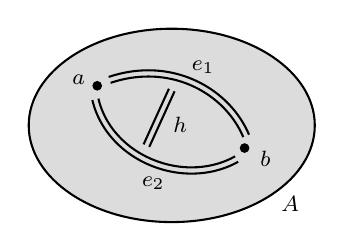
\begin{tikzpicture}[x=0.75pt,y=0.75pt,yscale=-1,xscale=1,roundnode/.style={circle, fill=black, inner sep=0pt, minimum size=3.5pt}]
    %uncomment if require: \path (0,300); %set diagram left start at 0, and has height of 300

    %Shape: Ellipse [id:dp3643970014729053] 
    \draw  [fill={rgb, 255:red, 220; green, 220; blue, 220 }  ,fill opacity=1 ] (4,52.08) .. controls (4,26.36) and (34.86,5.5) .. (72.92,5.5) .. controls (110.98,5.5) and (141.83,26.36) .. (141.83,52.08) .. controls (141.83,77.81) and (110.98,98.67) .. (72.92,98.67) .. controls (34.86,98.67) and (4,77.81) .. (4,52.08) -- cycle ;
    %Curve Lines [id:da06896022650610556] 
    \draw    (42.51,28.73) .. controls (49.06,26.53) and (55.48,25.53) .. (61.61,25.53) .. controls (81.63,25.53) and (98.59,36.2) .. (107.29,50.91) .. controls (108.37,52.74) and (109.33,54.63) .. (110.14,56.57)(43.46,31.57) .. controls (49.69,29.48) and (55.78,28.53) .. (61.61,28.53) .. controls (80.48,28.53) and (96.5,38.56) .. (104.71,52.44) .. controls (105.72,54.15) and (106.61,55.92) .. (107.38,57.73) ;
    %Curve Lines [id:da08140854638152761] 
    \draw    (37.58,39.19) .. controls (41.3,54.8) and (53.94,65.9) .. (68.57,70.27) .. controls (72.96,71.58) and (77.53,72.28) .. (82.1,72.31) .. controls (82.22,72.31) and (82.34,72.31) .. (82.46,72.31) .. controls (89.71,72.31) and (96.96,70.63) .. (103.45,66.99)(34.66,39.89) .. controls (38.64,56.55) and (52.07,68.48) .. (67.72,73.14) .. controls (72.37,74.53) and (77.23,75.28) .. (82.08,75.31) .. controls (82.2,75.31) and (82.33,75.31) .. (82.46,75.31) .. controls (90.22,75.31) and (97.97,73.5) .. (104.92,69.61) ;
    %Straight Lines [id:da7856762818241472] 
    \draw    (74.28,35.66) -- (62.08,62.46)(71.55,34.42) -- (59.35,61.22) ;

    \node[roundnode] (B0) at (37,33) {};
    \node (C0) at (28,30) {\footnotesize{$a$}};
    \node[roundnode] (B1) at (108,63) {};
    \node (C1) at (118,68) {\footnotesize{$b$}};
    \node (C2) at (88,24) {\footnotesize{$e_1$}};
    \node (C3) at (64,80) {\footnotesize{$e_2$}};
    \node (C4) at (77,52) {\footnotesize{$h$}};
    \node (C5) at (130,90) {\footnotesize{$A$}};
    \end{tikzpicture}
  \end{minipage}
  \begin{minipage}{0.4\textwidth}
  \[
    \begin{array}{l}
      A : \varType_i \\
      a : A \\
      b : A \\
      e_1 : \Indeq{A}{a}{b} \\
      e_2 : \Indeq{A}{a}{b} \\
      h : \Indeq{(\Indeq{A}{a}{b})}{e_1}{e_2}
    \end{array}
  \]
  \end{minipage}
  \caption{Graphical representation of a type with inhabitants and equalities}
\end{figure}
 
All in all, types do not really resemble sets anymore. 
% 
Voevodsky noticed that they are much closer to \emph{weak \( \infty \)-groupoids}, 
a higher categorical gadget that plays an important role in homotopy theory, 
the branch of math that studies spaces and their deformations.
% 
This is the starting point of \emph{homotopy type theory} (HoTT), a far-reaching analogy
between homotopy theory and intensional type theory with the univalence 
axiom~\cite{hottbook}.

In homotopy theory, we think of types as spaces. Inhabitants of a type 
play the role of its points, equalities between two terms correspond to paths
between the points, equalities between two equalities are continuous
deformations between the corresponding paths, and so on. 
% 
Naturally, functions between types are continuous in that they preserve
equalities, and isomorphisms correspond to homotopy equivalences.

Homotopy type theory also extends the notion of inductive type to 
\emph{higher inductive types} (HITs), which feature constructors for equalities
in addition to constructors for elements.
% 
HITs provide a variety of basic spaces, such as the circle, the sphere and
the torus, but also a remarkably well-behaved notion of quotient types.
% 
\sideremark{The quotients defined in terms of HITs are effective}
\[
\begin{array}{l}
\mathsf{Inductive}\enskip\mathsf{circle} : \varType_0\enskip := \\
\sep \quad \mathsf{base} \enskip : \enskip \mathsf{circle}\\
\sep \quad \mathsf{loop} \enskip : \enskip \Indeq{\mathsf{circle}}{\mathsf{base}}{\mathsf{base}} \\
\\
\mathsf{Inductive}\enskip\mathsf{quotient}\ (A : \varType_i)\ (R : A \to A \to \varType_i) : \varType_i\enskip := \\
\sep \quad \mathsf{emb} \enskip : \enskip A \to \mathsf{quotient}\ A\ R \\
\sep \quad \mathsf{quo} \enskip : \enskip \Depfun[a\ b]{A}{R\ a\ b \to \Indeq{...}{\mathsf{emb}\ a}{\mathsf{emb}\ b}} \\
\end{array}
\]

Using higher inductive types and the univalence axiom it becomes possible to 
prove a surprising amount of classical results from homotopy theory, rephrased
to talk about types and equality:
% 
in his PhD thesis, Brunerie managed to show that the fourth homotopy group of
the three-dimensional sphere has two elements~\sidecite{Brunerie16}.
% 
Since then, the HoTT community has developed extensive libraries of formalized
univalent mathematics in \Coq~\sidecite{Bauer:2017:HLF:3018610.3018615} and
\Agda~\sidecite{agda-unimath}.

However, homotopy type theory is not exactly computational. The univalence
axiom is, well, an axiom -- which means that the \( \mathsf{J} \) eliminator
will not reduce when applied to an isomorphism converted to an equality 
using univalence.
% 
Higher inductive types also block computation, because their elimination 
principles are simply postulated as axioms.
% 
This situation is all the more disappointing as the features introduced by HoTT
seem to follow the principles of constructive mathematics.

\paragraph*{Cubical Type Theory}
% 
Subsequently, the type theory community directed its attention to the
search for a computational interpretation of the univalent equality. 

In 2014, Bezem \etal built a model of the univalence axiom in a constructive 
set theory~\sidecite{BezemCoquandHuber14}.
% 
Their model interprets types as \emph{fibrant cubical sets}, a combinatorial
model of weak \( \infty \)-groupoids that lends itself well to a constructive
presentation.
% 
Although this model does not quite provide a computational interpretation of
univalence, it laid the groundwork.

This program came to fruition a year later with the introduction of \emph{cubical type theory}, an intensional 
type theory based on the insights provided by the fibrant cubical 
sets~\sidecite{cubicaltt}.
% 
Cubical type theory incorporates primitives from homotopy theory directly in 
the typing judgments, and provides them with adequate computation rules.
% 
With this additional structure, it becomes possible to derive the principle of 
univalence as a theorem, thereby getting an axiom-free univalent theory.
% 
On top of this, cubical type theory supports higher inductive types with
natural elimination principles and computation rules. 

In the years following its introduction, cubical type theory flourished into a 
vibrant field of research.
% 
Many variations of the original system have been studied on paper~\cite{AngiuliHouHarper18,ABCFHL}
and implemented in proof assistants~\cite{Cubicaltt, redtt} --
% 
among them, the \texttt{cubical} mode of the \Agda proof assistant~\sidecite{cubical-agda}
is without a doubt the most successful implementation, as it has set the stage for several 
large-scale formalization projects.
% 
On the side of the metatheoretical investication, Huber proved a canonicity 
result~\sidecite{Huber16}, and Sterling and Angiuli obtained a normalization result
\sidecite{sterling_normalization_cubical}.

% There are multiple variations and implementations of cubical type
% theory---the original formulation of \citet{CCHM} used an interval
% endowed with the structure of a \emph{De Morgan algebra} while the
% more recent \emph{cartesian} cubical type theories use an interval
% with less structure~\cite{AngiuliHouHarper18,ABCFHL}. All of the

\section{Contributions}

Recent attempts to design a type theory based on observational equality
are either lacking an algorithm for type checking~\sidecitet{sterling_et_al:LIPIcs:2019:10538}, or restricted to a single
universe and having computational properties only up to a
conjecture~\sidecitet{Altenkirch2019}. Indeed, the latter relies on computation
in an enriched version of \MLTT that features a universe of definitionally
proof-irrelevant types (noted hereafter $\sProp$) as recently proposed
by~\sidecitet{gilbert:hal-01859964}, along with a proof-irrelevant identity type
that supports a strong eliminator. This theory has not been justified yet,
and it has even been shown not to be normalizing in presence of
impredicativity~\sidecitet{lmcs:6606}.

Furthermore, Altenkirch \etal sketch a normalization proof for observational 
type theory by explaining how to simulate the reduction behavior 

Normalization ``proof'', canonicity from consistency, proof-irrelevant axioms 
are fine, heterogeneous equality.

McBride et al : Epigram 2

In this paper, we define \SetoidTT, the first extension of \MLTT +
$\sProp$ with an observational equality that satisfies UIP, funext
and propext, and supports quotient types and countably many universes
---with a proof of normalization and canonicity formalized in \Agda.\footnote{The formalization is available at
  \url{https://github.com/CoqHott/logrel-mltt/}, references to a
  particular file are done using \refAgda{}{myfile} which
  directly points to the corresponding file on github.}
%
Firstly, we remark that this theory can only be derived in a system with
some level of cumulativity, as it is required for certain
computation rules to be well-typed. This makes explicit some difficulties
that do not show up in previous works.
%
Second, we remark that our version of observational equality can be equipped
with two elimination principles: a notion of type cast (or coercion) for
proof-relevant types, and the standard eliminator of \MLTT for
proof-irrelevant types, thus making all the setoidal structure
derivable from the standard eliminator.
%
Funext and propext are obtained by specifying the right
computation rules for observational equality whereas UIP is obtained
for free by interpreting observational equality in $\sProp$.

The proof of normalization and canonicity is based on the use
of logical relations defined in \Agda using induction-recursion as
initially developed by \sidecitet{Abel:POPL2018} and later extended to
$\sProp$ by~\sidecitet{gilbert:hal-01859964}.
%
Compared to previous work on formalized normalization proofs, we have added the support
for a cumulative hierarchy with two universes, and we make a clear distinction
between inhabitants of proof-irrelevant types, which have no computational
behavior, and inhabitants of proof-relevant types, which do.
%
This key change allows us to add new principles in $\sProp$ without
having to supply them with a computational behavior, trivializing for
instance the management of higher coherences of the cubical interpretation.
%
In counterpart for this added flexibility, normalization does not directly
imply canonicity anymore, and a separate proof of consistency of the
theory is required to derive canonicity.
%
This proof is done by defining a model for \SetoidTT, but as
consistency is the only consequence that we need from the existence of
a model, the model can be defined in an extensional setting.

To illustrate the simplicity of extending \MLTT+$\sProp$ to \SetoidTT,
we have implemented a simple version in
\Agda using rewrite rules, as recently introduced
by~\sidecitet{taming_of_the_rew} (file \refAgdaRoot{setoid\_rr}). 


\subsection{Definitional Proof Irrelevance}

In dependent type theory, a sort \( \sProp \) is said to be
\emph{impredicative} if it is closed under dependent products over any index
type: for all types \( A \) and functions \( \tm{B}{A \to \sProp} \),
the dependent product \( \Depfun{A}{B\ x} \) is in \( \sProp \).
%
In particular, impredicativity allows the definition of self-referential propositions,
which quantify over the type \( \sProp \) of all propositions and may thus
be applied to themselves.
%
In addition to providing a tremendous amount of logical power, impredicativity is
a crucial ingredient in common mathematical constructions, such as
Tarski's fixed point theorem or lattice theory~\sidecite{paco}.
%
On the other side of the coin, a predicative hierarchy $(\varType_i)_{i \in \Nat}$
requires dependent products to inhabit a higher universe level
than their domain and codomain: for all types \( A : \varType_i \) and functions
\( \tm{B}{A \to \varType_j} \), the dependent product
\( \Depfun{A}{B\ x} \) is in \( \varType_{max(i,j)} \).
%
While the latter is easier to model, as the universes $\varType_i$ can be
constructed incrementally by induction on the level $i$, it results
in a theory that is less flexible in practice, whether the mention of
levels is explicit (as in \Agda) or implicit (as in \Coq).
%
Impredicative propositions make for an altogether
more comfortable framework, in which less universe levels have to
be dealt with.

While impredicativity is a prominent feature of the Calculus of
Constructions~\sidecite{Coquand-CC}, and by extension of \Coq, it is
absent from the standard presentation of Martin-Löf type theory
(\MLTT~\sidecite{MARTINLOF197573}), and not available in \Agda.
%
This reluctance may be explained by the sheer difficulty of designing models
to reason about impredicative theories, and by the numerous incompatibility
results, from \sidecitet{hurkens95} paradox to the more recent proof by
\sidecitet{lmcs:6606} that a naive implementation of uniqueness of identity
proofs (UIP) via definitionally proof-irrelevant equalities breaks \Coq's
normalization algorithm on impredicative propositions.

However, as noted by Abel and Coquand, it is not clear whether that last
result stems from a deep incompatibility between UIP and impredicativity,
or if it is an artifact of an inadequate type-checking algorithm.
%
Clarifying this issue seems especially important given the renewed
interest in definitional proof-irrelevance and UIP shown by the community
in recent years~\sidecite{sterling_et_al:LIPIcs:2019:10538,pujet:hal-03367052,Altenkirch2019}.
%
For instance, the recent presentation \SetoidTT of observational
equality of \sidecitet{pujet:hal-03367052} has an equality which can be
eliminated using a cast operator that computes differently from the
usual eliminator of Martin-Löf identity type, as used by \sidecitet{lmcs:6606}.


In this paper, we show that impredicativity is harmless when confined
to a sort of definitionally proof-irrelevant propositions, as it is never
necessary to compute with irrelevant proof terms.
%
As a result, we are able to extend \SetoidTT with impredicativity while
preserving definitional UIP and all extensionality principles that come
with an observational type theory (such as propositional or function
extensionality).
%
The resulting system, dubbed \SetoidCC, still enjoys
normalization via inductive-recursive logical relations---no
realizability model is needed---and decidability of type-checking.
%
This result has been formalized in \Agda using the framework of
\sidecitet{Abel:POPL2018}.\footnote{see anonymous supplementary
  materials.}
%
The fact that a proof scheme that has been designed with predicative
theories in mind carries through in an impredicative setting
may come as a surprise.
%
The crux of the proof is to realize that we can get away with
remarkably little structure in the interpretation of the impredicative
dependent products and sums, to the extent that we do not even mention the
interpretation of the domain and codomain.
%
We manage to prove the soundness of our normalization model
despite this weaker induction hypothesis by using a \emph{paranoid}
version of the type system, which can then be proven equivalent to the
\emph{economic} version (a terminology introduced by
\sidecitet{andrej17:paranoid}).

%
Furthermore, we prove that normalization for \SetoidCC can be
carried in plain Martin-Löf type theory with indexed inductive types,
thereby showing that this impredicative universe does not contribute
to the computational power of the proof-relevant fragment at all,
despite the increase in logical power.
%
We also investigate the possibility of recovering the lost computational power
from a proof-relevant impredicative universe, hoping that the different
computational behaviour of \SetoidCC would allow us to circumvent Abel and
Coquand's argument, but alas, it does not. In fact, a slightly modified
argument shows undecidability of type-checking in presence of a
proof-relevant impredicative universe.
%
Therefore, we exhibit a tradeoff between the additional comfort of
UIP and extensionality principles, or the possibility to compute with
impredicative functions.

Finally, because our normalization proof does not imply logical
consistency, we define a model of \SetoidCC in ZF Set
theory.
%
This shows that the computational content of \SetoidCC can be studied
without impredicativity in the metatheory, while the study of the
logical content of \SetoidCC fundamentally requires impredicativity in
the metatheory. 


\section{Related work}

Compared to~\sidecite{altenkirchAl:plpv2007}, the most important ingredient in \SetoidTT is the
use of definitional proof-irrelevance.
%
This added flexibility in computations allows our recursors to enjoy proper computational
behavior on open terms, and it also lets us seamlessly treat universe hierarchies.
%
Moreover, the normalization proof for OTT relies on a normalization conjecture for a different
theory, unlike the normalization proof for \SetoidTT.

In~\sidecite{Altenkirch2019}, the authors define a setoid model in \( \MLTT+\sProp \). Then, they
interpret a version of \MLTT with proof-irrelevant identity types that support propext and
funext in their model, thereby providing a computational interpretation of these principles.
%
However, handling universes in their model requires some additions to \( \MLTT+\sProp \), and
the resulting theory is only conjectured to be normalizing.
%
In contrast to this, \SetoidTT is a full-fledged type theory and does not require any external
model to compute.

Compared to XTT~\sidecite{sterling_et_al:LIPIcs:2019:10538}, the strengths of \SetoidTT are a
normalization strategy that exhibits canonicity, as well a full proof that conversion and typing
are decidable. These properties allow us to present a concrete implementation of our system
in a proof assistant.
%
In XTT however, Sterling\etal show that typing cannot be decidable, as there is no way to deduce
\( \Obseq{A}{A'} \) and \( \Obseq{B}{B'} \) from a proof of \( \Obseq{A \times B}{A' \times B'} \).
%
In order to fix this shortcoming, they suggest adding a ``typecase'' operator, but
argue against it since it forces the universe to be closed, thereby severely constraining the
possible semantics.
%
In \SetoidTT, we obtain the injectivity of type contructors from the behavior of observational
equality in the universe. These rules somewhat constrain the semantics---for instance, we cannot
interpret \SetoidTT in set theory using a Grothendieck universe as the interpretation of \( \Type \)---but our universe remains open to the addition of arbitrary types.

\section{to put somewhere}

Allais and McBride on computation on refl

Bob atkey on observational equality that does not reduce

impossible to have canonicity for equality

inductive equality is predicative

explain the n+4

\sideremark{The \Coq proof assistant extends to the base calculus
of constructions
Predicative Calculus of Cumulative Inductive Constructions \cite{pcuic}}

Mixing type coercion operators and impredicative propositions is well known to 
be a minefield:
% % 
% in his seminal work on System F, Girard already shows that adding an operator 
% \( {J : \forall A\ B\ .\ A \to B} \) with the reduction rule
% \( {J\ A\ A\ t \Rightarrow t} \) breaks normalization \sidecite{girard72}.
in recent years, Coquand and Abel showed that the interaction of the two features 
breaks normalization in the type theory of \Lean \sidecite{lmcs:6606}.
% 
Still, they leave an open question: is there a way to decide conversion without

% And does the same argument applies to the observational equality of \SetoidCC, 
% which computes in a different way?
 
% As we will see, the answers to those questions are respectively ``no'' and 
% ``yes''.